\chapter{Bitcoin Scripting}

Le transazioni reali nella rete Bitcoin possiedono una struttura dati cruda (\textit{raw data}) complessa e standardizzata, spesso rappresentata in formati simil-JSON per facilitarne la lettura da parte degli sviluppatori.

\begin{figure}[H]
    \centering
    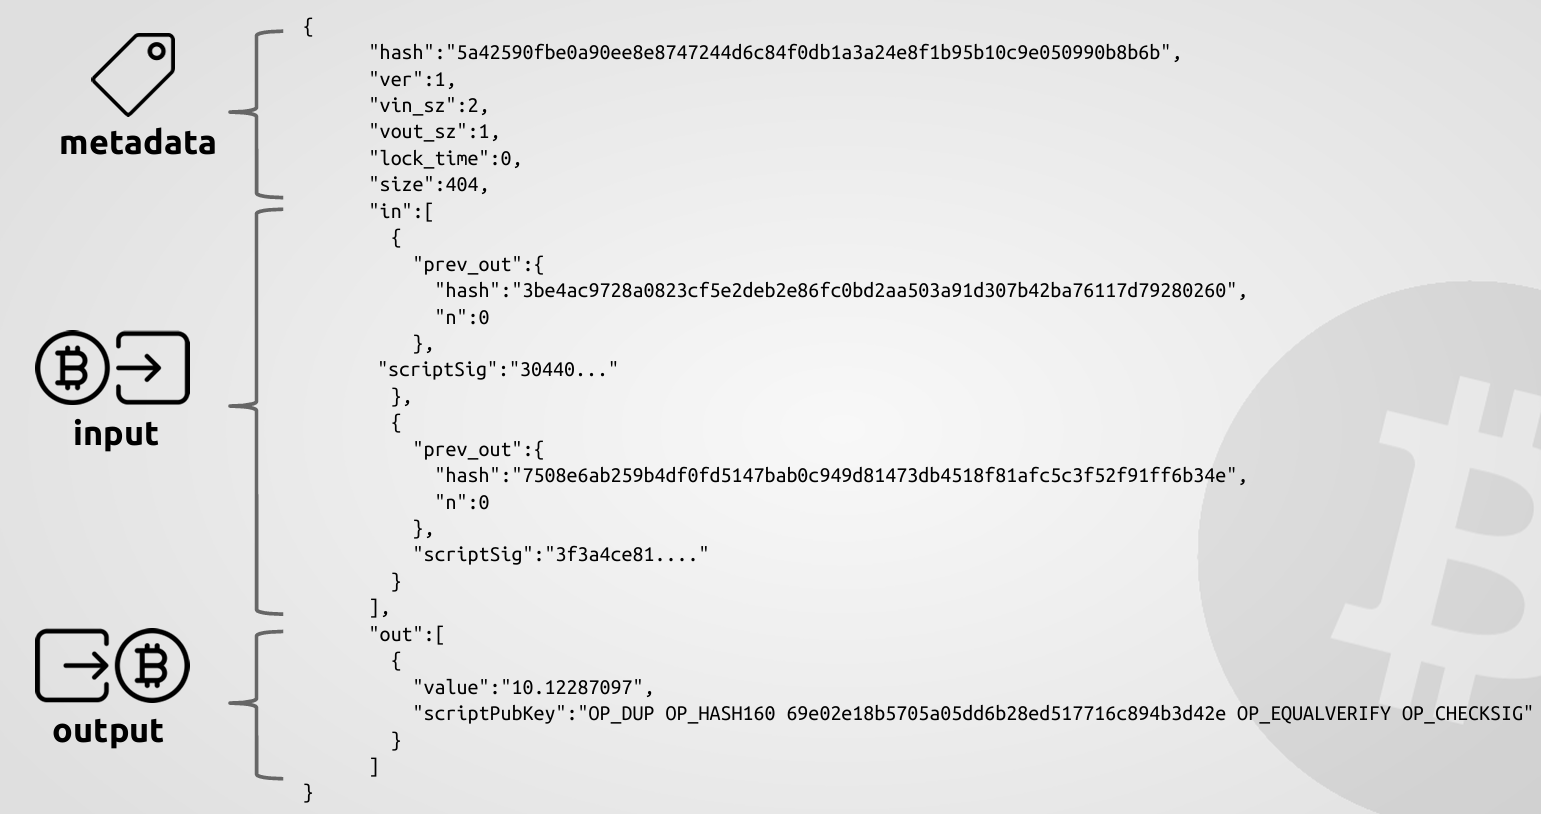
\includegraphics[width=1\linewidth]{Images/capitolo_2/trans_real.png}
\end{figure}

Come si evince dall'immagine, una transazione è divisa in tre sezioni logiche principali:

\begin{itemize}
    \item \textbf{Metadati:} Informazioni di servizio generali come l'hash della transazione stessa (TXID), la versione del protocollo e il \textit{locktime} che è il momento prima del quale la transazione non può essere inclusa in un blocco.
    
    \item \textbf{Inputs:} Contengono il riferimento ai fondi che si vogliono spendere.
    \begin{itemize}
        \item \textbf{\textit{prev\_out}:} È l'\textit{hash pointer} che punta univocamente all'UTXO di una transazione precedente. Contiene il TXID precedente e l'indice (\textit{n}) dello specifico output all'interno di quella transazione.
        \item \textbf{\textit{scriptSig}:} Conosciuto anche come \textbf{Unlocking Script}, è la componente crittografica che fornisce la prova di possesso dei fondi. Contiene la \textbf{firma digitale} e la \textbf{chiave pubblica di colui che possiede l'UTXO}. 
    \end{itemize}
    
    \item \textbf{Outputs:} Definiscono dove andranno i fondi e a quali condizioni.
    \begin{itemize}
        \item \textbf{\textit{value}:} La quantità di bitcoin trasferiti, espressa in \textit{satoshi} (la più piccola unità di Bitcoin, pari a $10^{-8}$ BTC).
        \item \textbf{\textit{scriptPubKey}:} Conosciuto anche come \textbf{Locking Script}, 
        contiene l'\textbf{indirizzo del destinatario} che non è altro che l'hash della sua chiave pubblica e, soprattutto, le condizioni logiche necessarie affinché questi fondi possano essere spesi in futuro.
    \end{itemize}
\end{itemize}

L'utilizzo dei termini "script" non è casuale. Il controllo sulla spesa dei Bitcoin non è affidato a una semplice verifica di saldi, ma all'esecuzione di veri e propri algoritmi scritti in \textbf{Bitcoin Script.}

\section*{Firma di un Input e del TXID}

Volendo riassumere in modo rigoroso il processo di firma e la definizione dell'identificativo della transazione, per ogni input che si desidera spendere avviene quanto segue:
\begin{enumerate}
    \item \textbf{Preparazione (Svuotamento e Sostituzione):} Si crea una copia temporanea della transazione in cui tutti i campi \texttt{scriptSig} vengono svuotati. Successivamente, esclusivamente nell'input che si sta validando, si inserisce temporaneamente lo \texttt{scriptPubKey} dell'UTXO di origine al posto di scriptSig.
    \item \textbf{Hashing temporaneo e Firma:} Si calcola l'hash di questa transazione temporanea per ottenere il \textit{Transaction Digest}. Questo hash rappresenta il "messaggio" che viene effettivamente firmato crittograficamente utilizzando la chiave privata dell'utente.
    \item \textbf{Assemblaggio finale:} Si scarta l'hash temporaneo appena calcolato. La firma digitale ottenuta al passo precedente, accompagnata dalla chiave pubblica in chiaro, viene inserita definitivamente nel campo \texttt{scriptSig} della transazione \textit{originale}.
    \item \textbf{Calcolo del TXID e Trasmissione:} A questo punto la transazione è completa e pronta per essere trasmessa (in \textit{broadcast}) alla rete. Il \textbf{TXID} (Transaction ID) viene calcolato dai nodi applicando un doppio SHA-256 all'intera transazione finale. È fondamentale ricordare che il TXID \textit{non} viene inserito come campo all'interno dei dati della transazione, ma funge esclusivamente da "impronta digitale" usata dal network per identificarla univocamente nella blockchain.
\end{enumerate}

\section{Il linguaggio Bitcoin Script}
Bitcoin Script è un linguaggio di scripting semplice, basato su una struttura dati a \textbf{pila} (pila o \textit{stack}). È progettato appositamente per essere sicuro e prevedibile:

\begin{itemize}
    \item \textbf{Nessuna memoria (\textit{stateless}):} L'esecuzione di uno script non ha memoria delle esecuzioni precedenti. Non esistono parametri di stato salvati.
    \item \textbf{Non Turing-completo:} Il linguaggio manca intenzionalmente di costrutti per cicli infiniti (come \texttt{for} o \texttt{while}), garantendo che ogni script termini la sua esecuzione in un tempo prevedibile, prevenendo attacchi di tipo \textit{Denial of Service} (DoS) ai nodi della rete.
\end{itemize}
Con questo linguaggio di scripting è possibile effettuare controlli su \textbf{firme multiple con threshold} o \textbf{proof of burn}.

\subsection{Il processo di validazione: Sblocco e Blocco}
Il cuore della sicurezza di Bitcoin risiede nel meccanismo con cui un input valida la spesa di un output precedente. Per verificare se una transazione ha il diritto di spendere un determinato UTXO, il network non esegue un solo script, ma combina lo script di sblocco dell'input attuale con lo script di blocco dell'output precedente.

\begin{figure}[H]
    \centering
    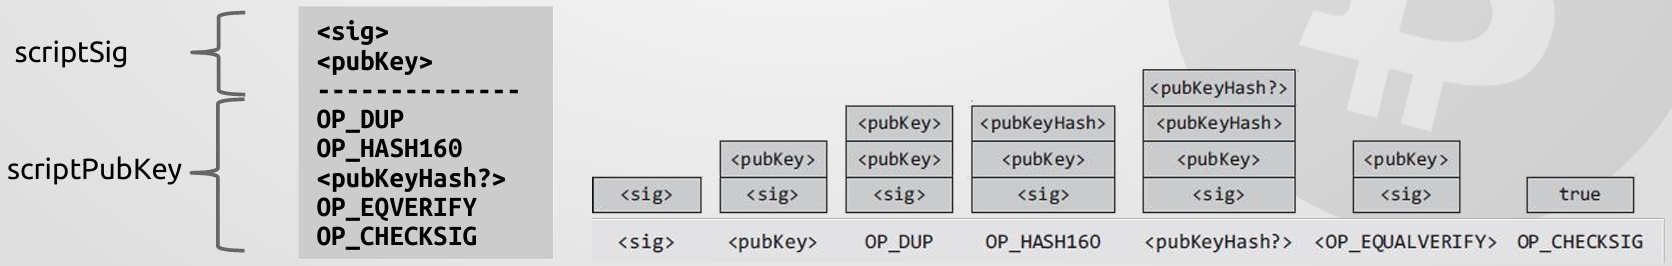
\includegraphics[width=1\linewidth]{Images/capitolo_2/verifica_firma.png}
\end{figure}

Come mostrato nel diagramma, il processo di valutazione standard (ad esempio per una transazione di tipo \textit{Pay-to-Public-Key-Hash} o P2PKH) avviene seguendo questi passi logici:

\begin{enumerate}
    \item \textbf{Esecuzione dell'Unlocking Script:} I nodi prendono lo \textbf{scriptSig} dall'input della transazione attuale. Questo script contiene la firma digitale e la chiave pubblica. Questi elementi vengono caricati (\textit{push}) sulla pila uno dopo l'altro.
    
    \item \textbf{Esecuzione del Locking Script:} Subito dopo, senza ripulire la pila, i nodi eseguono lo \textbf{scriptPubKey} prelevato dall'UTXO precedente che si vuole spendere. Questo script contiene una serie di operazioni logiche (opcodes) e l'hash dell'indirizzo del destinatario originale.
    
    \item \textbf{Verifica Crittografica (Passi logici):} Durante l'esecuzione combinata, lo script esegue due controlli fondamentali per garantire che il mittente sia l'autentico proprietario dei fondi:
    \begin{itemize}
        \item \textbf{Corrispondenza della Chiave Pubblica:} Lo scriptPubKey estrae la chiave pubblica fornita nello scriptSig, ne calcola l'hash e verifica che questo hash corrisponda esattamente all'hash dell'indirizzo salvato nello script di blocco originale. Questo assicura che la chiave pubblica fornita sia quella corretta.
        \item \textbf{Verifica della Firma:} Infine, lo scriptPubKey utilizza la chiave pubblica appena verificata per validare la firma digitale crittografica (anch'essa fornita nello scriptSig). Questa firma deve essere stata creata matematicamente a partire dai dati della transazione attuale, dimostrando che il mittente possiede la chiave privata corrispondente e che la transazione non è stata alterata.
    \end{itemize}
\end{enumerate}

Se, al termine dell'esecuzione di entrambe le parti dello script combinato, la pila contiene un singolo elemento non nullo (interpretato come "Vero" o 1), la transazione è considerata crittograficamente valida e può essere propagata nella rete e inclusa in un blocco. In caso contrario, è scartata.

\subsection{Multi Signatures con Threshold}
Come abbiamo già visto, Bitcoin permette di spendere fondi provenienti da più UTXO a patto che si possa provare, tramite apposita firma, la proprietà di ognuno di essi. Abbiamo definito questo caso come un \textbf{pagamento congiunto} poiché, in termini pratici, gli UTXO possono appartenere a persone diverse e servono quindi le firme di tutti i coinvolti per autorizzare l'operazione.

Un caso particolare è il sistema di \textbf{Multi Signatures con Threshold}. Tramite questa operazione, facciamo sì che un singolo UTXO sia vincolato a un gruppo di chiavi pubbliche, ma possa essere speso fornendo solo un numero minimo di firme (la soglia o threshold) rispetto al totale delle chiavi presenti. Ad esempio, una tipica multi-signature potrebbe elencare 5 chiavi pubbliche nell'UTXO, ma per spendere i fondi ne basterebbero solo 3, indipendentemente da quali siano i firmatari tra i 5 autorizzati.

Esiste inoltre la possibilità che un UTXO richieda la firma di tutti i suoi proprietari per poter essere speso. Possiamo definire questa situazione come un caso specifico di \textbf{Multi Signature con threshold N-su-N}, dove per muovere i fondi è necessaria la firma di tutti coloro che possiedono le chiavi associate all'UTXO, senza alcuna eccezione.

È chiaro che in questo scenario il rischio aumento poiché se anche una sola di queste chiavi viene persa, o se uno dei partecipanti si rifiuta di collaborare, l'UTXO diventa permanentemente bloccato e i fondi non potranno più essere recuperati in alcun modo.

\subsection{Proof-of-Burn}
La \textbf{Proof-of-Burn} è un'operazione mediante la quale è possibile letteralmente \textbf{buttare soldi}. Esistono principalmente due modi per farlo: il primo consiste nell'inviare i fondi a un cosiddetto \textbf{burn address}, ovvero un indirizzo di cui matematicamente nessuno possiede (o può generare) la chiave privata; il secondo è l'utilizzo dell'operazione \textit{OP\_RETURN}, che permette di contrassegnare un output come non spendibile a priori, consentendo però di aggiungere una piccola quantità di dati alla blockchain.

Questa è una pratica che nel contesto puro di Bitcoin ha poco senso, poiché ha come unico effetto quello di distruggere valuta. Tuttavia, viene utilizzata per scopi specifici come il \textbf{bootstrap} di una nuova moneta (dimostrando di aver "sacrificato" valore reale per ottenerla) o per il \textbf{timestamping}, ovvero usare la blockchain come un registro notarile per certificare l'esistenza di un dato in una certa data.

\subsection{Timestamping}
Il sistema di \textbf{Timestamping} permette di utilizzare la blockchain di Bitcoin come un registro notarile immutabile. Attraverso l'inserimento dell'hash di un documento all'interno di una transazione (spesso sfruttando l'operazione \textit{OP\_RETURN}), è possibile dimostrare con certezza assoluta che tale file esisteva già in una specifica data, certificata dal timestamp del blocco che contiene la transazione.

Inoltre, la flessibilità dello Script consente l'inserimento di quelli che vengono chiamati \textbf{Easter Eggs}: messaggi, citazioni o dati arbitrari nascosti all'interno della catena. Questa pratica, iniziata da Satoshi Nakamoto con il messaggio nel blocco genesi, serve a lasciare una traccia indelebile di informazioni non finanziarie direttamente nel registro distribuito.

\subsection{Real-life transaction con Escrow}
Un problema classico derivante dal sistema Bitcoin è quello dei pagamenti online tra parti che non si fidano l'una dell'altra. Supponiamo che $A$ voglia acquistare un bene da $B$: $A$ non vuole rischiare di inviare i soldi e non ricevere nulla, mentre $B$ non vuole spedire l'oggetto senza la garanzia di essere pagato. Questa situazione di stallo è nota in computer security come il problema dell'\textbf{Equa compravendita}.Per risolvere questa impasse, introduciamo una terza parte fidata, un \textbf{trusted third party} che chiameremo Giudice ($J$). La soluzione consiste nel creare una transazione con \textbf{multi signature a threshold 2-su-3} tra $A$, $B$ e $J$. In questo modo i fondi vengono "bloccati" in un UTXO che richiede almeno due firme per essere speso:
\begin{itemize}
    \item \textbf{Caso standard:} Se l'ordine arriva correttamente, $A$ e $B$ firmano insieme e i soldi vanno a $B$. Il giudice non interviene.
    \item \textbf{Caso di disputa:} Se nasce un problema, il giudice $J$ analizza le prove. Se dà ragione ad $A$, firmerà insieme ad $A$ per restituirgli i soldi (reso); se dà ragione a $B$, firmerà insieme a $B$ per completare il pagamento.
\end{itemize}
L'aspetto fondamentale è che il giudice $J$, pur avendo il potere di decidere l'esito della disputa, non può mai scappare con i soldi da solo, poiché la soglia di firme richiesta è 2 e lui ne possiede soltanto una.

\subsection{Micro-pagamenti e Lightning Network}
Supponiamo che $A$ e $B$ vogliano scambiarsi pagamenti frequenti, ad esempio per un servizio di chiamata tariffato al minuto. Effettuare una transazione sulla blockchain per ogni singolo minuto sarebbe insostenibile: i tempi di conferma sono lunghi e le commissioni (fees) per i miner supererebbero probabilmente il valore del pagamento stesso.Per risolvere questo problema, sfruttiamo il \textbf{lock\_time} combinato con una \textbf{multi-signature 2-su-2}. Il processo si divide in tre fasi:
\begin{enumerate}
    \item \textbf{Apertura del canale:} $A$ prepara una transazione di finanziamento (funding) che blocca una somma in un output richiedente le firme di entrambi ($A$ e $B$). \textbf{Attenzione:} prima di pubblicare questa transazione, $A$ si fa firmare da $B$ una transazione di \textbf{rescue} (con un \textit{lock\_time} futuro) che gli restituirebbe l'intero importo se il canale dovesse bloccarsi.
    \item \textbf{Scambio off-chain:} Durante la chiamata, $A$ invia a $B$ delle "micro\-transazioni" cumulative. Queste transazioni sono firmate solo da $A$, quindi non sono ancora valide per la rete. Ad ogni minuto, $A$ aggiorna la transazione assegnando a $B$ una quota maggiore e a se stesso (come resto) una quota minore.
    \item \textbf{Chiusura:} Alla fine della chiamata, $B$ prende l'ultima transazione ricevuta (quella con l'importo totale corretto), appone la sua firma e la pubblica sulla blockchain.
\end{enumerate}
$B$ è tranquillo perché ha in mano una transazione che può riscuotere in qualsiasi momento. $A$ è tranquillo perché, se $B$ dovesse sparire per non farlo cooperare, basterebbe attendere la scadenza del \textit{lock\_time} per riprendersi i soldi tramite la transazione di rescue. Una volta che la transazione finale viene pubblicata da $B$, quella di rescue diventa automaticamente nulla, poiché tenterebbe di spendere un UTXO che è già stato consumato (evitando così il \textit{double-spending}).

\subsection{Freezing Funds}
Supponiamo che $A$ voglia mettere da parte una certa somma di Bitcoin per il futuro, ad esempio come fondo di risparmio per un figlio, oppure che voglia semplicemente "auto-imporsi" di non spendere i propri fondi per un determinato periodo di tempo. In una transazione standard, chiunque possieda la chiave privata può muovere i fondi in qualsiasi momento; tuttavia, Bitcoin permette di "congelare" letteralmente un UTXO grazie all'istruzione \textit{OP\_CHECKLOCKTIMEVERIFY}.
Tramite questa operazione, facciamo sì che l'output della transazione non sia solo vincolato a una firma, ma anche a una condizione temporale specifica (espressa in data o in altezza del blocco). 
In pratica, lo script dell'UTXO dirà: "Questi soldi possono essere spesi solo se viene fornita la firma di $A$ \textbf{E} se il tempo trascorso è superiore a $X$".Naturalmente, questa condizione è scritta sulla blockchain e verificata dai nodi, il che la rende inviolabile: anche se $A$ possiede la chiave privata, se prova a spendere i fondi prima della scadenza, la rete rifiuterà la transazione considerandola invalida.
Questa funzione è fondamentale non solo per il risparmio a lungo termine, ma anche per la sicurezza di protocolli complessi. Come abbiamo visto nei micro-pagamenti, il sistema di "congelamento" permette di creare delle vie d'uscita (le transazioni di \textit{rescue}): se una controparte smette di collaborare, i fondi non restano bloccati per sempre nel limbo della multi-signature, ma ritornano automaticamente al proprietario originale una volta che il "tempo di blocco" è scaduto.
\subsection{Pay-to-Script-Hash (P2SH)}
Tutte le funzionalità che abbiamo analizzato finora, come le multi-signature o i sistemi di lock\_time, hanno un "difetto" naturale: rendono lo script di pagamento estremamente lungo e complesso. Se un venditore B chiedesse a un acquirente A di pagare verso uno script così complicato, A si ritroverebbe a dover inserire una mole enorme di dati nell'output della transazione, pagando di conseguenza commissioni molto più alte ai miner.

Per risolvere questo problema, utilizziamo il sistema \textbf{Pay-to-Script-Hash (P2SH)}. In questo scenario, immaginiamo che gli script complessi siano gestiti interamente dal venditore B. Invece di inviare a A l'intero set di istruzioni, B crea prima lo script (chiamato \textit{redeem script}), ne calcola l'\textbf{hash} e invia solo quest'ultimo ad A.

Questa procedura garantisce diversi vantaggi:
\begin{itemize}
    \item \textbf{Efficienza:} Lo \textit{scriptPubKey} rimane molto piccolo perché contiene solo l'hash dello script. Questo rende la transazione d'acquisto economica per A, indipendentemente dalla complessità delle regole imposte da B.
    \item \textbf{Sicurezza:} Il venditore deve generare l'hash e "pubblicarlo" (fornendolo ad A) prima del pagamento. In questo modo, B non può più modificare le condizioni dello script per provare a "barare", poiché se cambiasse anche una sola virgola dello script originale, l'hash non corrisponderebbe più e i fondi risulterebbero bloccati.
\end{itemize}

In pratica, i soldi rimangono bloccati nell'hash finché B non decide di spenderli. Solo in quel momento, all'interno dello \textit{scriptSig}, B dovrà fornire sia lo script completo che tutte le firme necessarie per farlo girare. La rete Bitcoin verificherà prima che lo script corrisponda all'hash e poi eseguirà le istruzioni per autorizzare il pagamento.
